
\section{Polyakov Representation of the Linking Number}
Consider a link made of two strands, $L_{1}$ and $L_{2}$. Consider the double line integral
\begin{equation*}
\Phi ( L_{1} ,L_{2}) =\frac{\epsilon _{ijk}}{4\pi }\oint _{L_{1}}\mathrm{d} x^{i}\oint _{L_{2}}\mathrm{d} y^{j}\frac{x^{k} -y^{k}}{|\boldsymbol{x} -\boldsymbol{y} |^{3}}
\end{equation*}
\begin{enumerate}
\item Show that $\Phi $ is equal to the phase accumulated by letting a unit of flux run along one strand, and moving a unit charged particle along the path of the other strand.
\item Show that the resulting phase is the topological invariant known as the linking number - the number of times one strand wraps around the other, see section 2.6.2.
\end{enumerate}

This integral representation of linking was known to Gauss.


\paragraph{Answer}

(a) According to the text, the path integral of the system is given by:
\begin{equation*}
Z=\sum _{\text{paths }\{\boldsymbol{x}( t)\}}\int \mathcal{D} a_{\mu }\exp\left(\frac{\mathrm{i}}{\hbar } S_{CS} +\frac{\mathrm{i} q}{\hbar }\int \mathrm{d} \ell ^{\alpha } a_{\alpha }\right) .
\end{equation*}
Integrate out $a_{\mu }$, we get a phase
\begin{equation*}
\sum _{\text{paths }\{\boldsymbol{x}( t)\}}\mathrm{e}^{\mathrm{i} S_{0} /\hbar }\mathrm{e}^{\mathrm{i} \theta W(\text{paths} )} .
\end{equation*}
We want to prove that
\begin{equation*}
2\pi \Phi ( L_{1} ,L_{2}) \varpropto \theta W( L_{1} ,L_{2}) .
\end{equation*}
In this case, the path dependent terms is given by
\begin{equation*}
\begin{aligned}
Z & =\int \mathcal{D} a_{\mu }\exp\left[\frac{\mathrm{i}}{\hbar }\oint _{L_{1}}\mathrm{d} \ell _{1}^{\alpha } a_{\alpha }\right]\exp\left[\frac{\mathrm{i}}{\hbar }\oint _{L_{2}}\mathrm{d} \ell _{2}^{\alpha } a_{\alpha }\right]\mathrm{e}^{\mathrm{i} S_{CS} /\hbar } .\\
 & \equiv \int \mathcal{D} a_{\mu } W_{1} W_{2}\mathrm{e}^{\mathrm{i} S_{CS} /\hbar } .
\end{aligned}
\end{equation*}
Here $W_{1} ,W_{2}$ denote the Wilson loop. The EOM we have got in the text is
\begin{equation*}
j^{\alpha } =\epsilon ^{\alpha \beta \gamma } \partial _{\beta } a_{\gamma } .
\end{equation*}
In Lorenz gauge, the solution is obtained in classical electrodynamics:
\begin{equation*}
a_{\alpha }( x) =\int \mathrm{d}^{3} y\epsilon _{\alpha \beta \gamma }\frac{\partial ^{\beta } j^{\gamma }( y)}{| \boldsymbol{x} -\boldsymbol{y}| } .
\end{equation*}
In this case, the flux is
\begin{equation*}
j_{a}^{\alpha } =\oint _{L_{a}}\mathrm{d} x_{a}^{\alpha } \delta (x-x_{a}( t) ),
\end{equation*}
then
\begin{equation*}
a_{\alpha }( x) =\sum _{a=1}^{2}\oint _{L_{a}}\mathrm{d} x_{a}^{\beta } \epsilon _{\alpha \beta \gamma }\frac{(x-x_{a} )^{\rho }}{| \boldsymbol{x} -\boldsymbol{x}_{a}| ^{3}} .
\end{equation*}
Therefore, the phase is given by:
\begin{equation*}
\begin{aligned}
Z & =\langle W_{1} W_{2} \rangle \\
 & =\exp(\mathrm{i} S_{CS}[ a_{\alpha }( x)])\\
 & =\exp\left(\frac{\mathrm{i}}{2\hbar }\oint _{L_{1}}\mathrm{d} x^{i}\oint _{L_{2}}\mathrm{d} y^{j} \epsilon _{ijk}\frac{x^{k} -y^{k}}{|\boldsymbol{x} -\boldsymbol{y} |^{3}}\right) =\exp\left(\frac{2\pi \mathrm{i}}{\hbar } \Phi ( L_{1} ,L_{2})\right) .
\end{aligned}
\end{equation*}


(b) Consider this two strands case. Using Stokes' theorem:
\begin{equation*}
\begin{aligned}
\Phi  & =\frac{1}{4\pi }\oint _{L_{1}}\mathrm{d} x^{i}\oint _{L_{2}}\mathrm{d} y^{j} \epsilon _{ijk}\frac{\partial }{\partial y_{k}}\left(\frac{1}{| \boldsymbol{x} -\boldsymbol{y}| }\right)\\
 & =\frac{1}{4\pi }\oint _{L_{1}}\mathrm{d} x^{i}\int _{\Sigma ( L_{2})}\mathrm{d}^{2} y_{i}\boldsymbol{\nabla }^{2}\left(\frac{1}{| \boldsymbol{x} -\boldsymbol{y}| }\right)\\
 & =\oint _{L_{1}}\mathrm{d} x^{i}\int _{\Sigma ( L_{2})}\mathrm{d}^{2} y_{i} \delta (\boldsymbol{x} -\boldsymbol{y}) .
\end{aligned}
\end{equation*}
Here $\Sigma ( L_{2})$ is an arbitrary surface bounded by $L_{2}$. Using the limit definition of $\delta $ function:
\begin{equation*}
\delta (\boldsymbol{x} -\boldsymbol{y}) =\lim _{\epsilon \rightarrow 0} \delta _{\epsilon }(\boldsymbol{x} -\boldsymbol{y}) =\lim _{\epsilon \rightarrow 0}\frac{1}{( 2\pi \epsilon )^{3/2}}\mathrm{e}^{-(\boldsymbol{x} -\boldsymbol{y})^{2} /\epsilon } .
\end{equation*}
Parameterize the $\epsilon \rightarrow 0$ region, we have 
\begin{equation*}
\Phi =\frac{1}{2\pi }\oint _{L_{1}}\mathrm{d} x^{i}( t) \epsilon _{ijk} n^{j}\dot{n}^{k} ,
\end{equation*}
where
\begin{equation*}
\dot{n}^{i} =\frac{\mathrm{d} n^{i}}{\mathrm{d} t} ,
\end{equation*}
and $n^{i}$ is the normal vector along the surface $\Sigma ( L_{2})$. Note here the integral is equal to $\mathrm{d}\boldsymbol{x} \cdot (\boldsymbol{n} \times \dot{\boldsymbol{n}} )$, which means the volume of the parallelepiped spanned by $\mathrm{d}\boldsymbol{x} ,\boldsymbol{n} ,\dot{\boldsymbol{n}}$, as Fig.\ref{fig:geometricMeaningOfPhi} shows.

\begin{figure}[h!]
\centering
\tikzset{every picture/.style={line width=0.75pt}} %set default line width to 0.75pt        

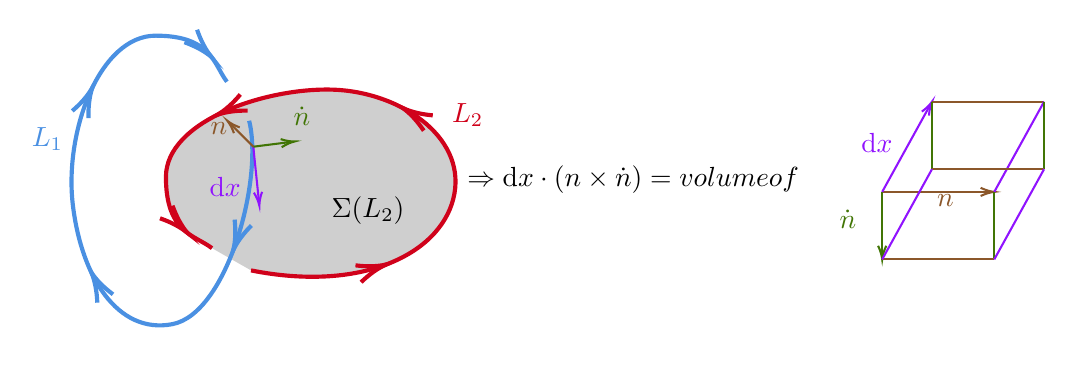
\begin{tikzpicture}[x=0.75pt,y=0.75pt,yscale=-1,xscale=1]
%uncomment if require: \path (0,149); %set diagram left start at 0, and has height of 149

%Curve Lines [id:da8583132747605609] 
\draw [color={rgb, 255:red, 208; green, 2; blue, 27 }  ,draw opacity=1 ][fill={rgb, 255:red, 155; green, 155; blue, 155 }  ,fill opacity=0.48 ][line width=1.5]    (194.61,117.89) .. controls (249.61,128.89) and (287.61,108.89) .. (292.61,80.89) .. controls (297.61,52.89) and (265.79,31.72) .. (233.7,30.8) .. controls (201.61,29.89) and (153.61,45.89) .. (153.61,72.89) .. controls (153.61,99.89) and (167.61,100.89) .. (175.81,107.19) ;
\draw [shift={(259.77,115.05)}, rotate = 161.65] [color={rgb, 255:red, 208; green, 2; blue, 27 }  ,draw opacity=1 ][line width=1.5]    (14.21,-4.28) .. controls (9.04,-1.82) and (4.3,-0.39) .. (0,0) .. controls (4.3,0.39) and (9.04,1.82) .. (14.21,4.28)   ;
\draw [shift={(267.76,39.67)}, rotate = 30.5] [color={rgb, 255:red, 208; green, 2; blue, 27 }  ,draw opacity=1 ][line width=1.5]    (14.21,-4.28) .. controls (9.04,-1.82) and (4.3,-0.39) .. (0,0) .. controls (4.3,0.39) and (9.04,1.82) .. (14.21,4.28)   ;
\draw [shift={(178.32,42.96)}, rotate = 335.28] [color={rgb, 255:red, 208; green, 2; blue, 27 }  ,draw opacity=1 ][line width=1.5]    (14.21,-4.28) .. controls (9.04,-1.82) and (4.3,-0.39) .. (0,0) .. controls (4.3,0.39) and (9.04,1.82) .. (14.21,4.28)   ;
\draw [shift={(163.88,99.74)}, rotate = 224.63] [color={rgb, 255:red, 208; green, 2; blue, 27 }  ,draw opacity=1 ][line width=1.5]    (14.21,-4.28) .. controls (9.04,-1.82) and (4.3,-0.39) .. (0,0) .. controls (4.3,0.39) and (9.04,1.82) .. (14.21,4.28)   ;
%Curve Lines [id:da39300436286828844] 
\draw [color={rgb, 255:red, 74; green, 144; blue, 226 }  ,draw opacity=1 ][line width=1.5]    (193.7,45.8) .. controls (200.7,73.8) and (183.14,138.77) .. (156.7,143.8) .. controls (130.26,148.84) and (112.7,120.8) .. (108.7,85.8) .. controls (104.7,50.8) and (121.7,4.8) .. (148.7,4.8) .. controls (175.7,4.8) and (176.7,18.8) .. (183,27) ;
\draw [shift={(186.02,108.25)}, rotate = 289.44] [color={rgb, 255:red, 74; green, 144; blue, 226 }  ,draw opacity=1 ][line width=1.5]    (14.21,-4.28) .. controls (9.04,-1.82) and (4.3,-0.39) .. (0,0) .. controls (4.3,0.39) and (9.04,1.82) .. (14.21,4.28)   ;
\draw [shift={(117.68,118.87)}, rotate = 62.09] [color={rgb, 255:red, 74; green, 144; blue, 226 }  ,draw opacity=1 ][line width=1.5]    (14.21,-4.28) .. controls (9.04,-1.82) and (4.3,-0.39) .. (0,0) .. controls (4.3,0.39) and (9.04,1.82) .. (14.21,4.28)   ;
\draw [shift={(118.17,29.83)}, rotate = 114] [color={rgb, 255:red, 74; green, 144; blue, 226 }  ,draw opacity=1 ][line width=1.5]    (14.21,-4.28) .. controls (9.04,-1.82) and (4.3,-0.39) .. (0,0) .. controls (4.3,0.39) and (9.04,1.82) .. (14.21,4.28)   ;
\draw [shift={(175.55,15.07)}, rotate = 225.37] [color={rgb, 255:red, 74; green, 144; blue, 226 }  ,draw opacity=1 ][line width=1.5]    (14.21,-4.28) .. controls (9.04,-1.82) and (4.3,-0.39) .. (0,0) .. controls (4.3,0.39) and (9.04,1.82) .. (14.21,4.28)   ;
%Straight Lines [id:da06655701164023453] 
\draw [color={rgb, 255:red, 144; green, 19; blue, 254 }  ,draw opacity=1 ]   (195.7,58.3) -- (198.43,84.78) ;
\draw [shift={(198.64,86.77)}, rotate = 264.11] [color={rgb, 255:red, 144; green, 19; blue, 254 }  ,draw opacity=1 ][line width=0.75]    (6.56,-1.97) .. controls (4.17,-0.84) and (1.99,-0.18) .. (0,0) .. controls (1.99,0.18) and (4.17,0.84) .. (6.56,1.97)   ;
%Straight Lines [id:da6327116286471945] 
\draw [color={rgb, 255:red, 65; green, 117; blue, 5 }  ,draw opacity=1 ]   (195.7,58.3) -- (213.66,56.03) ;
\draw [shift={(215.64,55.77)}, rotate = 172.77] [color={rgb, 255:red, 65; green, 117; blue, 5 }  ,draw opacity=1 ][line width=0.75]    (6.56,-1.97) .. controls (4.17,-0.84) and (1.99,-0.18) .. (0,0) .. controls (1.99,0.18) and (4.17,0.84) .. (6.56,1.97)   ;
%Straight Lines [id:da6514808042987321] 
\draw [color={rgb, 255:red, 139; green, 87; blue, 42 }  ,draw opacity=1 ]   (195.7,58.3) -- (184.55,47.16) ;
\draw [shift={(183.14,45.74)}, rotate = 45] [color={rgb, 255:red, 139; green, 87; blue, 42 }  ,draw opacity=1 ][line width=0.75]    (6.56,-1.97) .. controls (4.17,-0.84) and (1.99,-0.18) .. (0,0) .. controls (1.99,0.18) and (4.17,0.84) .. (6.56,1.97)   ;

%Straight Lines [id:da40116566849742963] 
\draw [color={rgb, 255:red, 139; green, 87; blue, 42 }  ,draw opacity=1 ]   (498.7,80.07) -- (550.7,80.07) ;
\draw [shift={(552.7,80.07)}, rotate = 180] [color={rgb, 255:red, 139; green, 87; blue, 42 }  ,draw opacity=1 ][line width=0.75]    (6.56,-1.97) .. controls (4.17,-0.84) and (1.99,-0.18) .. (0,0) .. controls (1.99,0.18) and (4.17,0.84) .. (6.56,1.97)   ;
%Straight Lines [id:da12682825681341425] 
\draw [color={rgb, 255:red, 65; green, 117; blue, 5 }  ,draw opacity=1 ]   (498.7,80.07) -- (498.7,110.6) ;
\draw [shift={(498.7,112.6)}, rotate = 270] [color={rgb, 255:red, 65; green, 117; blue, 5 }  ,draw opacity=1 ][line width=0.75]    (6.56,-1.97) .. controls (4.17,-0.84) and (1.99,-0.18) .. (0,0) .. controls (1.99,0.18) and (4.17,0.84) .. (6.56,1.97)   ;
%Straight Lines [id:da11570457898035436] 
\draw [color={rgb, 255:red, 144; green, 19; blue, 254 }  ,draw opacity=1 ]   (498.7,80.07) -- (521.73,38.35) ;
\draw [shift={(522.7,36.6)}, rotate = 118.9] [color={rgb, 255:red, 144; green, 19; blue, 254 }  ,draw opacity=1 ][line width=0.75]    (6.56,-1.97) .. controls (4.17,-0.84) and (1.99,-0.18) .. (0,0) .. controls (1.99,0.18) and (4.17,0.84) .. (6.56,1.97)   ;
%Straight Lines [id:da01686158483804845] 
\draw [color={rgb, 255:red, 139; green, 87; blue, 42 }  ,draw opacity=1 ]   (522.7,36.6) -- (576.7,36.6) ;
%Straight Lines [id:da7041284654080007] 
\draw [color={rgb, 255:red, 144; green, 19; blue, 254 }  ,draw opacity=1 ]   (552.7,80.07) -- (576.7,36.6) ;
%Straight Lines [id:da5204493055002457] 
\draw [color={rgb, 255:red, 65; green, 117; blue, 5 }  ,draw opacity=1 ]   (522.7,36.6) -- (522.7,69.12) ;
%Straight Lines [id:da5677138120668197] 
\draw [color={rgb, 255:red, 65; green, 117; blue, 5 }  ,draw opacity=1 ]   (576.7,36.6) -- (576.7,69.12) ;
%Straight Lines [id:da043969288075480506] 
\draw [color={rgb, 255:red, 65; green, 117; blue, 5 }  ,draw opacity=1 ]   (552.7,80.07) -- (552.7,112.6) ;
%Straight Lines [id:da6691056719845112] 
\draw [color={rgb, 255:red, 139; green, 87; blue, 42 }  ,draw opacity=1 ]   (498.7,112.6) -- (552.7,112.6) ;
%Straight Lines [id:da2667372097560283] 
\draw [color={rgb, 255:red, 139; green, 87; blue, 42 }  ,draw opacity=1 ]   (522.7,69.12) -- (576.7,69.12) ;
%Straight Lines [id:da3644682999290392] 
\draw [color={rgb, 255:red, 144; green, 19; blue, 254 }  ,draw opacity=1 ]   (498.7,112.6) -- (522.7,69.12) ;
%Straight Lines [id:da9775456056327838] 
\draw [color={rgb, 255:red, 144; green, 19; blue, 254 }  ,draw opacity=1 ]   (552.7,112.6) -- (576.7,69.12) ;


% Text Node
\draw (297.32,66.1) node [anchor=north west][inner sep=0.75pt]    {$\mathrm{\Rightarrow d}\boldsymbol{x} \cdot (\boldsymbol{n} \times \dot{\boldsymbol{n}} )=\text{volume of}$};
% Text Node
\draw (476.64,87.27) node [anchor=north west][inner sep=0.75pt]  [color={rgb, 255:red, 65; green, 117; blue, 5 }  ,opacity=1 ]  {$\dot{\boldsymbol{n}}$};
% Text Node
\draw (523.64,79.77) node [anchor=north west][inner sep=0.75pt]  [color={rgb, 255:red, 139; green, 87; blue, 42 }  ,opacity=1 ]  {$\boldsymbol{n}$};
% Text Node
\draw (487.14,50.27) node [anchor=north west][inner sep=0.75pt]  [color={rgb, 255:red, 144; green, 19; blue, 254 }  ,opacity=1 ]  {$\mathrm{d}\boldsymbol{x}$};
% Text Node
\draw (87.5,47.5) node [anchor=north west][inner sep=0.75pt]  [color={rgb, 255:red, 74; green, 144; blue, 226 }  ,opacity=1 ]  {$L_{1}$};
% Text Node
\draw (290,36) node [anchor=north west][inner sep=0.75pt]  [color={rgb, 255:red, 208; green, 2; blue, 27 }  ,opacity=1 ]  {$L_{2}$};
% Text Node
\draw (232,81) node [anchor=north west][inner sep=0.75pt]    {$\Sigma ( L_{2})$};
% Text Node
\draw (173.14,71.5) node [anchor=north west][inner sep=0.75pt]  [color={rgb, 255:red, 144; green, 19; blue, 254 }  ,opacity=1 ]  {$\mathrm{d}\boldsymbol{x}$};
% Text Node
\draw (213.64,37.5) node [anchor=north west][inner sep=0.75pt]  [color={rgb, 255:red, 65; green, 117; blue, 5 }  ,opacity=1 ]  {$\dot{\boldsymbol{n}}$};
% Text Node
\draw (173.64,45) node [anchor=north west][inner sep=0.75pt]  [color={rgb, 255:red, 139; green, 87; blue, 42 }  ,opacity=1 ]  {$\boldsymbol{n}$};
\end{tikzpicture}
\caption{The geometric meaning of $\Phi $.}
\label{fig:geometricMeaningOfPhi}
\end{figure}

Therefore due to $\boldsymbol{n} \perp \dot{\boldsymbol{n}}$ in this two loop case, we have
\begin{equation*}
\Phi =\frac{1}{2\pi }\oint _{L_{1}} \epsilon \mathrm{d} \theta =\epsilon ,
\end{equation*}
where $\epsilon =1$ or $-1$ depend on the relative direction whether $\mathrm{d}\boldsymbol{x}$ is in the same direction as $\boldsymbol{n} \times \dot{\boldsymbol{n}}$. In the case of Fig.\ref{fig:geometricMeaningOfPhi}, $\epsilon =1$ according to the right handed rule. This is exactly the definition using the sign of the crossing:$( \epsilon ( L_{1}) +\epsilon ( L_{2}))) /2$.

For the prove in the general case, you can refer to \cite{ricca2011gauss}. 
\section{Gauge Transforming the Chern-Simons Action}
Make the gauge transform Eq. 5.13 on the Chern-Simons action $5.9$ and show that it results in the change 5.15. Note that there will be an additional term that shows up which it a total derivative and will therefore vanish when integrated over the whole manifold $\mathcal{M}$.

\paragraph{Answer}
We first give the transformation rule of the general Chern-Simons action. Under the gauge transformation:
\begin{equation*}
\mathrm{d} a_{\mu }\rightarrow \mathrm{d} (U^{-1}\mathrm{d} U+U^{-1} a_{\mu } U)=\mathrm{d} U^{-1}\mathrm{\land d} U+\mathrm{d} U^{-1} \land a_{\mu } U+U^{-1}\mathrm{d} a_{\mu } U-U^{-1} a_{\mu } \land \mathrm{d} U.
\end{equation*}
Using $\mathrm{d} U^{-1} =-U^{-1}\mathrm{d} U\land U^{-1}$, we have:
\begin{equation*}
\begin{aligned}
\mathrm{d} a_{\mu } & \rightarrow -U^{-1}\mathrm{d} U\land U^{-1} \land \mathrm{d} U-U^{-1}\mathrm{d} U\land U^{-1} \land a_{\mu } U+U^{-1}\mathrm{d} a_{\mu } U-U^{-1} a_{\mu } \land \mathrm{d} U\\
 & =-U^{-1}\mathrm{d} U\land a_{\mu } +U^{-1}\mathrm{d} a_{\mu } U-U^{-1} a_{\mu } \land \mathrm{d} U.
\end{aligned}
\end{equation*}
Under this transformation, consider the difference
\begin{equation*}
\begin{aligned}
 & \operatorname{tr}( a'_{\mu } \land \mathrm{d} a'_{\mu }) -\operatorname{tr}( a_{\mu } \land \mathrm{d} a_{\mu })\\
\rightarrow  & \operatorname{tr}\left[ (U^{-1}\mathrm{d} U+U^{-1} a_{\mu } U)\land (-U^{-1}\mathrm{d} U\land a_{\mu } +U^{-1}\mathrm{d} a_{\mu } U-U^{-1} a_{\mu } \land \mathrm{d} U)-a_{\mu } \land \mathrm{d} a_{\mu }\right]\\
= & \operatorname{tr}[\textcolor[rgb]{0.82,0.01,0.11}{-(U}\textcolor[rgb]{0.82,0.01,0.11}{^{-1}}\mathrm{\textcolor[rgb]{0.82,0.01,0.11}{d}}\textcolor[rgb]{0.82,0.01,0.11}{U)}\textcolor[rgb]{0.82,0.01,0.11}{^{2}}\textcolor[rgb]{0.82,0.01,0.11}{\land a'_{\mu }} -\textcolor[rgb]{0.29,0.56,0.89}{U^{-1}}\textcolor[rgb]{0.29,0.56,0.89}{a_{\mu } U\land U}\textcolor[rgb]{0.29,0.56,0.89}{^{-1}}\mathrm{\textcolor[rgb]{0.29,0.56,0.89}{d}}\textcolor[rgb]{0.29,0.56,0.89}{U\land a'_{\mu }} +U^{-1}\mathrm{d} U\land U^{-1}\mathrm{d} a_{\mu } U+\textcolor[rgb]{0.74,0.06,0.88}{U^{-1}}\textcolor[rgb]{0.74,0.06,0.88}{a_{\mu } U\land U}\textcolor[rgb]{0.74,0.06,0.88}{^{-1}\mathrm{d} a_{\mu } U}\\
 & \textcolor[rgb]{0.82,0.01,0.11}{-U}\textcolor[rgb]{0.82,0.01,0.11}{^{-1}}\mathrm{\textcolor[rgb]{0.82,0.01,0.11}{d}}\textcolor[rgb]{0.82,0.01,0.11}{U\land U}\textcolor[rgb]{0.82,0.01,0.11}{^{-1}}\textcolor[rgb]{0.82,0.01,0.11}{a_{\mu } U\land U}\textcolor[rgb]{0.82,0.01,0.11}{^{-1}}\mathrm{\textcolor[rgb]{0.82,0.01,0.11}{d}}\textcolor[rgb]{0.82,0.01,0.11}{U} -\textcolor[rgb]{0.29,0.56,0.89}{U^{-1}}\textcolor[rgb]{0.29,0.56,0.89}{a_{\mu } U\land U}\textcolor[rgb]{0.29,0.56,0.89}{^{-1}}\textcolor[rgb]{0.29,0.56,0.89}{a_{\mu } U\land U}\textcolor[rgb]{0.29,0.56,0.89}{^{-1}}\mathrm{\textcolor[rgb]{0.29,0.56,0.89}{d}}\textcolor[rgb]{0.29,0.56,0.89}{U} -\textcolor[rgb]{0.74,0.06,0.88}{a_{\mu } \land }\mathrm{\textcolor[rgb]{0.74,0.06,0.88}{d}} a_{\mu }]\\
= & \operatorname{tr}\left[\textcolor[rgb]{0.82,0.01,0.11}{-(U}\textcolor[rgb]{0.82,0.01,0.11}{^{-1}}\mathrm{\textcolor[rgb]{0.82,0.01,0.11}{d}}\textcolor[rgb]{0.82,0.01,0.11}{U)}\textcolor[rgb]{0.82,0.01,0.11}{^{2}}\textcolor[rgb]{0.82,0.01,0.11}{\land (a'_{\mu } +U}\textcolor[rgb]{0.82,0.01,0.11}{^{-1}}\textcolor[rgb]{0.82,0.01,0.11}{a_{\mu } U)} -\textcolor[rgb]{0.29,0.56,0.89}{U^{-1}}\textcolor[rgb]{0.29,0.56,0.89}{a_{\mu } U\land U}\textcolor[rgb]{0.29,0.56,0.89}{^{-1}}\mathrm{\textcolor[rgb]{0.29,0.56,0.89}{dU\land }}\textcolor[rgb]{0.29,0.56,0.89}{(a'_{\mu } +U}\textcolor[rgb]{0.29,0.56,0.89}{^{-1}}\textcolor[rgb]{0.29,0.56,0.89}{a_{\mu } U)} +U^{-1}\mathrm{d} U\land U^{-1}\mathrm{d} a_{\mu } U\right] .
\end{aligned}
\end{equation*}
The second term gives:
\begin{equation*}
\begin{aligned}
 & \frac{2}{3}\operatorname{tr} (a'{_{\mu }}^{3} -a_{\mu }^{3})\\
= & \frac{2}{3}\operatorname{tr}\left[ (U^{-1}\mathrm{d} U+U^{-1} a_{\mu } U)^{3} -a{_{\mu }}^{3}\right]\\
= & \operatorname{tr}\left[\frac{2}{3} (U^{-1}\mathrm{d} U)^{3} +\textcolor[rgb]{0.82,0.01,0.11}{2(U}\textcolor[rgb]{0.82,0.01,0.11}{^{-1}}\mathrm{\textcolor[rgb]{0.82,0.01,0.11}{d}}\textcolor[rgb]{0.82,0.01,0.11}{U)}\textcolor[rgb]{0.82,0.01,0.11}{^{2}}\textcolor[rgb]{0.82,0.01,0.11}{\land U}\textcolor[rgb]{0.82,0.01,0.11}{^{-1}}\textcolor[rgb]{0.82,0.01,0.11}{a_{\mu } U} +\textcolor[rgb]{0.29,0.56,0.89}{2U}\textcolor[rgb]{0.29,0.56,0.89}{^{-1}}\mathrm{\textcolor[rgb]{0.29,0.56,0.89}{d}}\textcolor[rgb]{0.29,0.56,0.89}{U\land (U}\textcolor[rgb]{0.29,0.56,0.89}{^{-1}}\textcolor[rgb]{0.29,0.56,0.89}{a_{\mu } U)}\textcolor[rgb]{0.29,0.56,0.89}{^{2}}\right] .
\end{aligned}
\end{equation*}
So the two terms gives:
\begin{equation*}
\begin{aligned}
 & \operatorname{tr}\left( a'_{\mu } \land \mathrm{d} a'_{\mu } +\frac{2}{3} a'{_{\mu }}^{3}\right) -\operatorname{tr}\left( a_{\mu } \land \mathrm{d} a_{\mu } +\frac{2}{3} a_{\mu }^{3}\right)\\
= & \operatorname{tr}\left\{\frac{2}{3} (U^{-1}\mathrm{d} U)^{3} +\textcolor[rgb]{0.82,0.01,0.11}{(U}\textcolor[rgb]{0.82,0.01,0.11}{^{-1}}\mathrm{\textcolor[rgb]{0.82,0.01,0.11}{d}}\textcolor[rgb]{0.82,0.01,0.11}{U)}\textcolor[rgb]{0.82,0.01,0.11}{^{2}}\textcolor[rgb]{0.82,0.01,0.11}{\land (U}\textcolor[rgb]{0.82,0.01,0.11}{^{-1}}\textcolor[rgb]{0.82,0.01,0.11}{a_{\mu } U-a'_{\mu } )} -\textcolor[rgb]{0.29,0.56,0.89}{U^{-1}}\textcolor[rgb]{0.29,0.56,0.89}{a_{\mu } U\land U}\textcolor[rgb]{0.29,0.56,0.89}{^{-1}}\mathrm{\textcolor[rgb]{0.29,0.56,0.89}{dU\land }}\textcolor[rgb]{0.29,0.56,0.89}{(U}\textcolor[rgb]{0.29,0.56,0.89}{^{-1}}\textcolor[rgb]{0.29,0.56,0.89}{a_{\mu } U-a'_{\mu } )}\right. \\
 & \left. + U^{-1}\mathrm{d} U\land U^{-1}\mathrm{d} a_{\mu } U\right\}\\
= & -\frac{1}{3}\operatorname{tr} (U^{-1}\mathrm{d} U)^{3} +\operatorname{tr}\left[ U^{-1}\mathrm{d} U\land (U^{-1}\mathrm{d} a_{\mu } U-\textcolor[rgb]{0.29,0.56,0.89}{U^{-1}}\mathrm{\textcolor[rgb]{0.29,0.56,0.89}{d}}\textcolor[rgb]{0.29,0.56,0.89}{U\land U}\textcolor[rgb]{0.29,0.56,0.89}{^{-1}}\textcolor[rgb]{0.29,0.56,0.89}{a_{\mu } U} )\right]\\
= & -\frac{1}{3}\operatorname{tr} (U^{-1}\mathrm{d} U)^{3} +\operatorname{tr}\left[\mathrm{d} (U^{-1} a_{\mu } U\land U^{-1}\mathrm{d} U)\right] .
\end{aligned}
\end{equation*}
So we have:
\begin{equation}
S_{CS}\rightarrow S_{CS} +\frac{k}{4\pi }\int _{M}\mathrm{d}\operatorname{tr} (U^{-1} a_{\mu } U\land U^{-1}\mathrm{d} U)-\frac{k}{12\pi }\int _{M}\operatorname{tr} ((U^{-1} dU)^{3} ).
\label{eq:gaugeTransformationOfCSAction}
\end{equation}
Now, we can specify that $M=S^{3}$, therefore, the second term vanishes because $S^{3}$ is closed. Then we consider the third term. Suppose $G=SU( 2) \cong S^{3}$, then we consider a function $U:S^{3}\rightarrow S^{3}$:
\begin{equation*}
( t_{1} ,t_{2} ,t_{3} ,t_{4}) \mapsto ( x_{1} ,x_{2} ,x_{3} ,x_{4}) .
\end{equation*}
Then we can use complex numbers $z=x_{1} +\mathrm{i} x_{2} ,w=x_{3} +\mathrm{i} x_{4}$ to characterize them. We can see $U$ can be expressed as:
\begin{equation*}
U=\begin{pmatrix}
z & -w\\
\bar{w} & \bar{z}
\end{pmatrix} ,| z| ^{2} +| w| ^{2} =1.
\end{equation*}
Noting that $\mu =U^{-1}\mathrm{d} U$ is the Maurer-Cartan form and $\operatorname{tr} (\mu \land \mu \land \mu )/6$ is the left-invariant volume form of $SU( 2)$, so the third term is propotional to the mapping degree of $U$, which indicate that it is an integer! Now let's start our proof.

The Maurer-Cartan form $U^{-1}\mathrm{d} U$ can be parametrized as:
\begin{equation*}
U^{-1}\mathrm{d} U=\begin{pmatrix}
\bar{z}\mathrm{d} z+w\mathrm{d}\bar{z} & -\bar{z}\mathrm{d} w+w\mathrm{d}\bar{z}\\
-\bar{w}\mathrm{d} z+z\mathrm{d}\bar{w} & \bar{w}\mathrm{d} w+z\mathrm{d}\bar{z}
\end{pmatrix} .
\end{equation*}
The condition $| z| ^{2} +| w| ^{2} =1$ gives
\begin{equation*}
\bar{w}\mathrm{d} w+z\mathrm{d}\bar{z} =-(\bar{z}\mathrm{d} z+w\mathrm{d}\bar{w}) .
\end{equation*}
If we call the basis $T^{i} \equiv \sigma ^{i} /2$, and call $\alpha \equiv -\bar{z}\mathrm{d} w+w\mathrm{d} z$, then we have:
\begin{equation*}
U^{-1}\mathrm{d} U=( \alpha -\bar{\alpha }) T^{1} +\mathrm{i}( \alpha +\bar{\alpha }) T^{2} +2(\bar{z}\mathrm{d} z+w\mathrm{d}\bar{w}) T^{3} \equiv a_{i} T^{i} \in \mathfrak{su}( 2) ,
\end{equation*}
which means the Maurer-Cartan form $U^{-1}\mathrm{d} U$ is an element of $\mathfrak{su}( 2)$ Lie algebra. Then we have:
\begin{equation*}
\begin{aligned}
\operatorname{tr} (U^{-1}\mathrm{d} U)^{3} & =a^{a} \land a^{b} \land a^{c}\operatorname{tr}( T^{a} T^{b} T^{c} )\\
 & =a^{a} \land a^{b} \land a^{c}\frac{1}{2}\operatorname{tr} [([T^{a} ,T^{b} ]+\{T^{a} ,T^{b} \})T^{c} ]\\
 & =\frac{1}{2} a^{a} \land a^{b} \land a^{c}\operatorname{tr}\left[\left(\mathrm{i} \epsilon ^{abc} T^{d} +\frac{\delta ^{ab}}{2}\right) T^{c}\right]\\
 & =\frac{\mathrm{i}}{2} \epsilon ^{abd} a^{a} \land a^{b} \land a^{c} =\frac{3\mathrm{i}}{2} a^{1} \land a^{2} \land a^{3} .
\end{aligned}
\end{equation*}
In terms of $z$ and $w$, we have:
\begin{equation*}
\begin{aligned}
\operatorname{tr} (U^{-1}\mathrm{d} U)^{3} = & \frac{3\mathrm{i}}{2}( \alpha -\bar{\alpha }) \land \mathrm{i}( \alpha +\bar{\alpha }) \land 2(\bar{z}\mathrm{d} z+w\mathrm{d}\bar{w})\\
= & 6( w\mathrm{d}\bar{z} -\bar{z}\mathrm{d} w) \land ( z\mathrm{d}\bar{w} -\bar{w}\mathrm{d} z) \land (\bar{z}\mathrm{d} z+w\mathrm{d}\bar{w})\\
= & 6( w\mathrm{d}\bar{z} \land \mathrm{d}\bar{w} \land \mathrm{d} z+\bar{z}\mathrm{d} w\land \mathrm{d} z\land \mathrm{d}\bar{w})\\
\xlongequal[w=x_{3} +\mathrm{i} x_{4}]{z=x_{1} +\mathrm{i} x_{2}} & -12\mathrm{i}[( x_{3} +\mathrm{i} x_{4})\mathrm{d} x_{1} \land \mathrm{d} x_{2} \land (\mathrm{d} x_{3} -\mathrm{id} x_{4}) -( x_{1} -\mathrm{i} x_{2})\mathrm{d} x_{3} \land \mathrm{d} x_{4} \land (\mathrm{d} x_{1} +\mathrm{id} x_{2})]\\
= & 12\sum _{i=1}^{4}( -1)^{i} x_{i}\mathrm{d} x_{1} \land \cdots \cdots \land \mathrm{d} x_{4}\\
- & 12\mathrm{i}[\mathrm{d} x_{1} \land \mathrm{d} x_{2} \land ( x_{3}\mathrm{d} x_{3} +x_{4}\mathrm{d} x_{4}) -( x_{1}\mathrm{d} x_{1} +x_{2}\mathrm{d} x_{2}) \land \mathrm{d} x_{3} \land \mathrm{d} x_{4}] .
\end{aligned}
\end{equation*}
But use
\begin{equation*}
| z| ^{2} +| w| ^{2} =1\Rightarrow \sum _{i=1}^{4} x_{i}\mathrm{d} x_{i} =0\Rightarrow x_{1}\mathrm{d} x_{1} +x_{2}\mathrm{d} x_{2} =-( x_{3}\mathrm{d} x_{3} +x_{4}\mathrm{d} x_{4}) ,
\end{equation*}
which means
\begin{equation*}
\operatorname{tr} (U^{-1}\mathrm{d} U)^{3} =12\sum _{i=1}^{4}( -1)^{i} x_{i}\mathrm{d} x_{1} \land \cdots \hat{\mathrm{d} x_{i}} \cdots \land \mathrm{d} x_{4} =12U^{*}\tilde{\omega } .
\end{equation*}
Where $\tilde{\omega }$ is the volume form of $S^{3}$, $U^{*}$ is the pull back of $U$. So according to the definition of mapping degree:
\begin{equation*}
\begin{aligned}
\frac{k}{12\pi }\int _{S^{3}}\operatorname{tr} (U^{-1}\mathrm{d} U)^{3} & =\frac{k}{\pi }\int _{S^{3}} U^{*}\tilde{\omega }\\
 & =\frac{k}{\pi }\deg U\cdot \int _{S^{3}}\tilde{\omega }\\
 & =\frac{k}{\pi }\deg U\int _{D^{4}} 4\mathrm{d} y^{1} \land \mathrm{d} y^{2} \land \mathrm{d} y^{3} \land \mathrm{d} y^{4}\\
 & =2\pi k\deg U.
\end{aligned}
\end{equation*}
Call $\deg U=\nu \in \mathbb{Z}$, we finally \ arrive our goal:
\begin{equation*}
S_{CS}\rightarrow S_{CS} +2\pi \nu k.
\end{equation*}
Furthermore, we can argue that the level $k$ \textbf{must} be an integer in order for the partition function to be well-defined. Because $a'_{\mu }$ and $a_{\mu }$ are connected by the \textbf{gauge} transformation, which means the partition function should not change:
\begin{equation*}
\mathrm{e}^{\mathrm{i} S[ a_{\mu }]}\stackrel{!}{=}\mathrm{e}^{\mathrm{i} S[ a'_{\mu }]} \Rightarrow S[ a_{\mu }] =S[ a'_{\mu }] +2k\pi ,k\in \mathbb{Z}.
\end{equation*}
This gives $k\cdot \deg U\in \mathbb{Z} \Rightarrow k\in \mathbb{Z}$. 

\section{Winding Numbers of Groups in Manifolds}
Consider the mapping of $U(x)\in SU(2)\rightarrow S^{3}$. Construct an example of a map with winding number $n$ for arbitrary $n$. I.e., find a representative of each group element of $\Pi _{3} (SU(2))$ (See note 17).

\paragraph{Answer}
Let's construct a kind of famous map: the hedgehog ansatz. This is a map with spherical symmetry:
\begin{equation*}
U_{H}( r) =\exp(\mathrm{i} F( r)\hat{\boldsymbol{r}} \cdot \boldsymbol{\sigma }) \in SU( 2) ,
\end{equation*}
Here $F( r)$ is an arbitrary function about $r$. In nucleon theory, this ansatz correspond to the pion field with spherical symmetry:
\begin{equation*}
\boldsymbol{\pi }( r) =F_{\pi } F( r)\hat{\boldsymbol{r}} ,
\end{equation*}
as the Fig.\ref{fig:hedgehog} shows, so this map is called the hedgehog ansatz. 
\begin{figure}[h!]
\centering
\includegraphics{hedgehog.pdf}
\caption{The hedgehog ansatz, the figure shows the diagram presentation of $\boldsymbol{\pi }$ field, the length of the arrow is proportional to $F( r)$.}
\label{fig:hedgehog}
\end{figure}

Now we try to determine the boundary condition of $F( r)$. We know $SU( 2) \cong S^{3} =\mathbb{R}^{3} \cup \{\infty \}$, we can set $U(| \boldsymbol{x}| \rightarrow \infty )=\mathds{1}$(this means the field becomes vacuum at the infinity physically), then we have
\begin{equation*}
F( \infty ) =0.
\end{equation*}
We can then expand $U_{H}$:
\begin{equation*}
U_{H}( r) =\cos F( r)\mathds{1} +\mathrm{i}\sin F( r)\hat{\boldsymbol{r}} \cdot \boldsymbol{\sigma } ,
\end{equation*}
which means $F$ is actually the azimuthal angle of the group space. At the origin, our field cannot have any `out-pointing' component, due to continuity. Therefore, our boundary condition must impose that $\sin F(0)=0$, which implies
\begin{equation*}
F(0)=n\pi ,\ \ n\in \mathbb{Z} .
\end{equation*}
With these two boundary condition, we can actually calculate the topological charge, i.e. the additional term in the gauge transformation \eqref{eq:gaugeTransformationOfCSAction} of $S_{CS}$:
\begin{equation*}
\mathcal{B} \equiv \operatorname{tr} ((U^{-1} \mathrm{d} U)^{3} )=\frac{1}{2\pi ^{2} r^{2}} F'( r)\sin^{2}( F( r)) ,
\end{equation*}
and the integration gives:
\begin{equation}
\begin{aligned}
B[ U_{H}] & \equiv \frac{1}{24\pi ^{2}} \epsilon _{ijk}\int \mathrm{d}^{3} x\operatorname{tr} ((U^{-1} \mathrm{d} U)^{3} )\\
 & =-\frac{2}{\pi }\int _{0}^{\infty } F'( r)\sin^{2} F\mathrm{d} r\\
 & =\frac{1}{\pi }\left. \left[\frac{1}{2}\sin 2F-F\right]\right| _{r=0}^{r\rightarrow \infty } =n\in \mathbb{Z} .
\end{aligned}
\label{eq:windingNumberOfU}
\end{equation}
Of course, we can also use the geometry method to compute $B$. Note that $S^{3}$ can be parameterized by three angles $( F,\Theta ,\Phi )$, and $B$ is the winding number of the map, which means we just need to pull back the normalized volume element on $S^{3}$ to the real space. The volume form of $S^{3}$ in $\mathbb{R}^{4}$ is given by
\begin{equation*}
\mathrm{d} \Omega =\sin^{2} F\sin\mathrm{\Theta d} F\land \mathrm{d} \Theta \land \mathrm{d} \Phi ,
\end{equation*}
and the integration gives
\begin{equation*}
\int \mathrm{d} \Omega =\int _{0}^{\pi }\sin^{2} F\mathrm{d} F\int _{0}^{\pi }\sin\mathrm{\Theta d} \Theta \int _{0}^{2\pi }\mathrm{d} \Phi =2\pi ^{2} ,
\end{equation*}
i.e. the normalized volume form is
\begin{equation*}
\hat{\mathrm{d} \Omega } =\frac{1}{2\pi ^{2}}\sin^{2} F\sin\mathrm{\Theta d} F\land \mathrm{d} \Theta \land \mathrm{d} \Phi .
\end{equation*}
Then we define the pull back to be:
\begin{equation*}
\left\{\begin{aligned}
F & \rightarrow F( r) \Rightarrow \mathrm{d} F=F'\mathrm{d} r\\
\Theta  & \rightarrow \theta \\
\Phi  & \rightarrow \phi ,
\end{aligned}\right. ,
\end{equation*}
then the integral in real space equals to
\begin{equation*}
\int _{\mathbb{R}^{3}}\tilde{\hat{\mathrm{d} \Omega }} =\frac{1}{2\pi ^{2}}\int _{\infty }^{0} F'\sin^{2} F\mathrm{d} r\int _{0}^{\pi }\sin \theta \mathrm{d}\int _{0}^{2\pi }\mathrm{d} \Phi ,
\end{equation*}
which will also give \eqref{eq:windingNumberOfU}.

\section{Quantization of Winding Number}
Let us consider the manifold $S^{3}$ which we consider as $\mathbb{R}^{3}$ plus a point at infinity. Consider the gauge transform function defined
\begin{equation*}
U(\boldsymbol{x} )=\exp\left(\frac{\mathrm{i} \pi N\boldsymbol{x} \cdot \boldsymbol{\sigma }}{\sqrt{|\boldsymbol{x} |^{2} +R^{2}}}\right)
\end{equation*}
where $\boldsymbol{x}$ is a point in $\mathbb{R}^{3}$, and $\boldsymbol{\sigma }$ represents the Pauli matrices with $R$ an arbitrary length scale. Show the winding number Eq. $5.16$ gives the integer $N$. Why does $N$ need to be an integer here?

\paragraph{Answer}
We can just repeat our calculation in our last calculation again. To throw away $N$, we consider $B[ U_{1} U_{2}]$. Write it down:
\begin{equation*}
B[ U_{1} U_{2}] =\frac{1}{24\pi ^{2}} \epsilon _{ijk}\int \mathrm{d}^{3} x\operatorname{tr} (U_{2}^{\dagger } U_{1}^{\dagger } \partial _{i}( U_{1} U_{2}) \partial _{j} (U_{2}^{\dagger } U_{1}^{\dagger } )\partial _{k}( U_{1} U_{2}) ).
\end{equation*}
where we have used the identity $( U_{1} U_{2})^{\dagger } \equiv U_{2}^{\dagger } U_{1}$.(Noting that $U$ is unitary, we can use $U^{\dagger }$ instead of $U^{-1}$). Expanding the traced part out yields
\begin{equation*}
\begin{aligned}
 & U_{2}^{\dagger } U_{1}^{\dagger }( \partial _{i} U_{1}) U_{2} (\partial _{j} U_{2}^{\dagger } )U_{1}^{\dagger }( \partial _{k} U_{1}) U_{2} & \text{ term } 1\\
+ & U_{2}^{\dagger } U_{1}^{\dagger }( \partial _{i} U_{1}) U_{2} (\partial _{j} U_{2}^{\dagger } )U_{1}^{\dagger }\textcolor[rgb]{0.82,0.01,0.11}{U_{1}( \partial _{k} U_{2})} & \text{ term } 2\\
+ & \cancel{U_{2}^{\dagger }} U_{1}^{\dagger }( \partial _{i} U_{1})\cancel{U_{2} U_{2}^{\dagger }} (\partial _{j} U_{1}^{\dagger } )( \partial _{k} U_{1})\cancel{U_{2}} & B[ U_{1}]\\
+ & U_{2}^{\dagger } U_{1}^{\dagger }( \partial _{i} U_{1}) U_{2} U_{2}^{\dagger } (\partial _{j} U_{1}^{\dagger } )U_{1}( \partial _{k} U_{2}) & \text{ term } 4\\
+ & U_{2}^{\dagger } U_{1}^{\dagger }\textcolor[rgb]{0.82,0.01,0.11}{U_{1}( \partial _{i} U_{2}) (\partial _{j} U_{2}^{\dagger } )U_{1}^{\dagger }( \partial _{k} U_{1}) U_{2}} & \text{ term } 5\\
+ & U_{2}^{\dagger }\cancel{U_{1}^{\dagger } U_{1}}( \partial _{i} U_{2}) (\partial _{j} U_{2}^{\dagger } )\cancel{U_{1}^{\dagger } U_{1}}( \partial _{k} U_{2}) & B[ U_{2}]\\
+ & U_{2}^{\dagger } U_{1}^{\dagger } U_{1}( \partial _{i} U_{2}) U_{2}^{\dagger } (\partial _{j} U_{1}^{\dagger } )( \partial _{k} U_{1}) U_{2} & \text{ term } 7\\
+ & U_{2}^{\dagger } U_{1}^{\dagger } U_{1}( \partial _{i} U_{2}) U_{2}^{\dagger } (\partial _{j} U_{1}^{\dagger } )\textcolor[rgb]{0.82,0.01,0.11}{U_{1}( \partial _{k} U_{2})} . & \text{ term } 8
\end{aligned}
\end{equation*}
Now we can integrate by part, for example, the red term in term 2 \ gives $U_{1}( \partial _{k} U_{2})\rightarrow -( \partial _{k} U_{1}) U_{2}$, which cancels term 1. Similarly, term 7 cancels term 8. Finally, in term 5 we can integrate by parts three times, which cancels term 4. Which means we have the additive property
\begin{equation*}
B[ U_{1} U_{2}] =B[ U_{1}] +B[ U_{2}] .
\end{equation*}
Then we can see
\begin{equation*}
B[ U(\boldsymbol{x})] =B[U_{1}(\boldsymbol{x})^{N} ]=NB[ U_{1}(\boldsymbol{x})] ,
\end{equation*}
where
\begin{equation*}
U_{1} (\boldsymbol{x} )=\exp\left(\frac{\mathrm{i} \pi \boldsymbol{x} \cdot \boldsymbol{\sigma }}{\sqrt{|\boldsymbol{x} |^{2} +R^{2}}}\right) .
\end{equation*}
Then we try to compute $B[ U_{1}]$. Expand first:
\begin{equation*}
U_{1}(\boldsymbol{x}) =\cos\left(\frac{\mathrm{i} \pi | \boldsymbol{x}| }{\sqrt{|\boldsymbol{x} |^{2} +R^{2}}}\right)\mathds{1} +\mathrm{i}\sin\left(\frac{\mathrm{i} \pi | \boldsymbol{x}| }{\sqrt{|\boldsymbol{x} |^{2} +R^{2}}}\right)\boldsymbol{n} \cdot \boldsymbol{\sigma } .
\end{equation*}
Where $\boldsymbol{n} =\boldsymbol{x} /| \boldsymbol{x}| $. We also embed the base space $S^{3}$ into $\mathbb{R}^{4}$ like before, while this time, we can use the coordinate
\begin{equation*}
y^{0} \equiv \cos\left(\frac{\mathrm{i} \pi | \boldsymbol{x}| }{\sqrt{|\boldsymbol{x} |^{2} +R^{2}}}\right) ,\quad \boldsymbol{y} =\sin\left(\frac{\mathrm{i} \pi | \boldsymbol{x}| }{\sqrt{|\boldsymbol{x} |^{2} +R^{2}}}\right)\boldsymbol{n} .
\end{equation*}
Then
\begin{equation*}
U_{1} \equiv y^{0}\mathds{1} +\boldsymbol{y} \cdot \boldsymbol{\sigma } ,
\end{equation*}
with the condition $(y^{0} )^{2} +\boldsymbol{y}^{2} =1$. The winding number clearly doesn't depend on the coordinate, we can use the point $y^{0} =1$, i.e. the north pole to evaluate $B$. Now
\begin{equation*}
\begin{aligned}
\mathcal{B}[ U_{1}] & =\operatorname{tr} ((U_{1}^{-1}\mathrm{d} U_{1} )^{3} )=\operatorname{tr} [(\mathrm{id}\boldsymbol{y} \cdot \boldsymbol{\sigma } )^{3} ]\\
 & =\mathrm{i}^{3} 3!\operatorname{tr}( \sigma _{1} \sigma _{2} \sigma _{3})\mathrm{d} y^{1} \land \mathrm{d} y^{2}\mathrm{\land d} y^{3}\\
 & =12\mathrm{d} y^{1} \land \mathrm{d} y^{2}\mathrm{\land d} y^{3} .
\end{aligned}
\end{equation*}
Then the integration over $\mathbb{R}^{3}$ gives
\begin{equation*}
B[ U_{1}] =\frac{1}{24\pi ^{2}} \times 12\times 2\pi ^{2} =1.
\end{equation*}
Finally, we can see
\begin{equation*}
B[ U(\boldsymbol{x})] =NB[ U_{1}] =N.
\end{equation*}
Besides, at the infinity, we have
\begin{equation*}
U(\boldsymbol{x}\rightarrow \infty )=\exp(\mathrm{i} \pi N\boldsymbol{n} \cdot \boldsymbol{\sigma }) ,
\end{equation*}
which should be independent of $\boldsymbol{n}$(or more physically, $U\rightarrow \mathds{1}$), which means $\sin( N\pi ) =0$, thus $N$ must be an integer. 
